% Fixture 7: pgfplots/TikZ with shadings, fadings and transparency. Renderer stress.
\documentclass[aspectratio=169]{beamer}
\usetheme{default}
\usepackage{pgfplots}
\pgfplotsset{compat=1.17}
\usepgfplotslibrary{fillbetween}
\usetikzlibrary{fadings,shadings,patterns}
\title{TikZ heavy}
\subtitle{Fixture 7}
\author{Lectern fixtures}
\date{}
\begin{document}
\begin{frame}
  \titlepage
\end{frame}
\begin{frame}{Line plots with fill between}
  \centering
  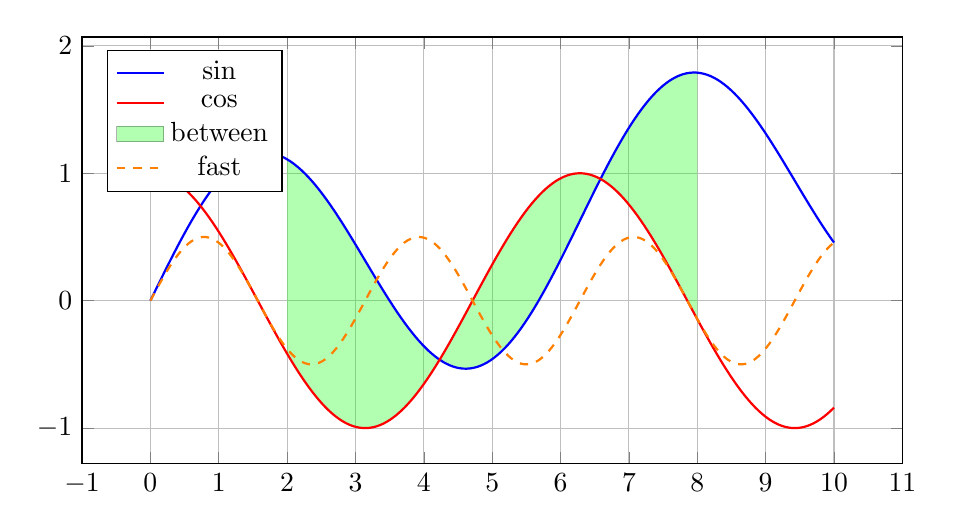
\begin{tikzpicture}
    \begin{axis}[width=12cm,height=7cm,grid=major,legend pos=north west,samples=200,domain=0:10]
      \addplot[name path=a,blue,thick] {sin(deg(x))+0.1*x};
      \addplot[name path=b,red,thick] {cos(deg(x))};
      \addplot[fill=green,opacity=0.3] fill between[of=a and b,soft clip={domain=2:8}];
      \addplot[orange,dashed,thick] {0.5*sin(deg(2*x))};
      \legend{sin,cos,between,fast}
    \end{axis}
  \end{tikzpicture}
\end{frame}
\begin{frame}{Surface with interpolated shading}
  \centering
  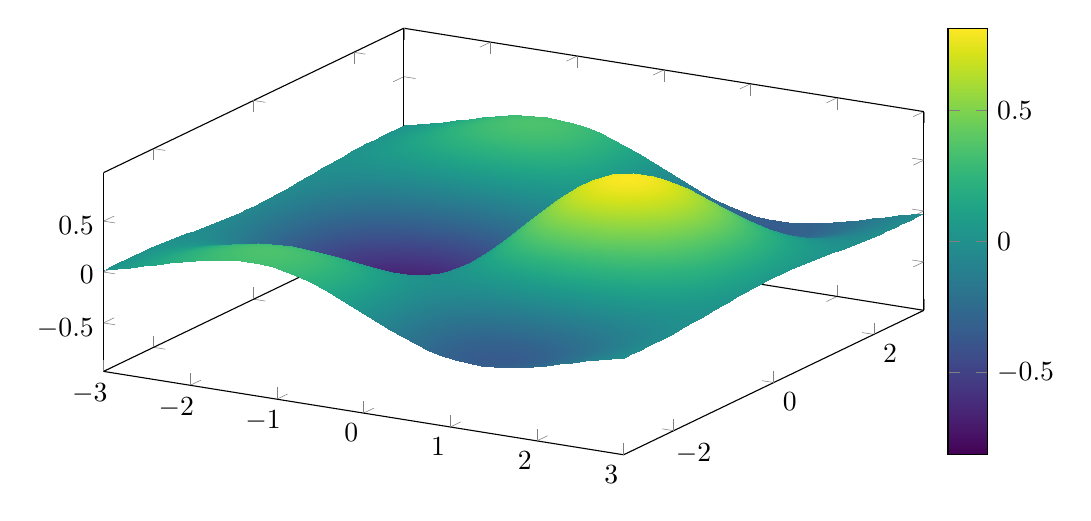
\begin{tikzpicture}
    \begin{axis}[width=12cm,height=7cm,view={30}{40},colormap/viridis,colorbar]
      \addplot3[surf,shader=interp,samples=41,domain=-3:3] {sin(deg(x))*cos(deg(y))*exp(-0.1*(x^2+y^2))};
    \end{axis}
  \end{tikzpicture}
\end{frame}
\begin{frame}{Shadings and fadings}
  \centering
  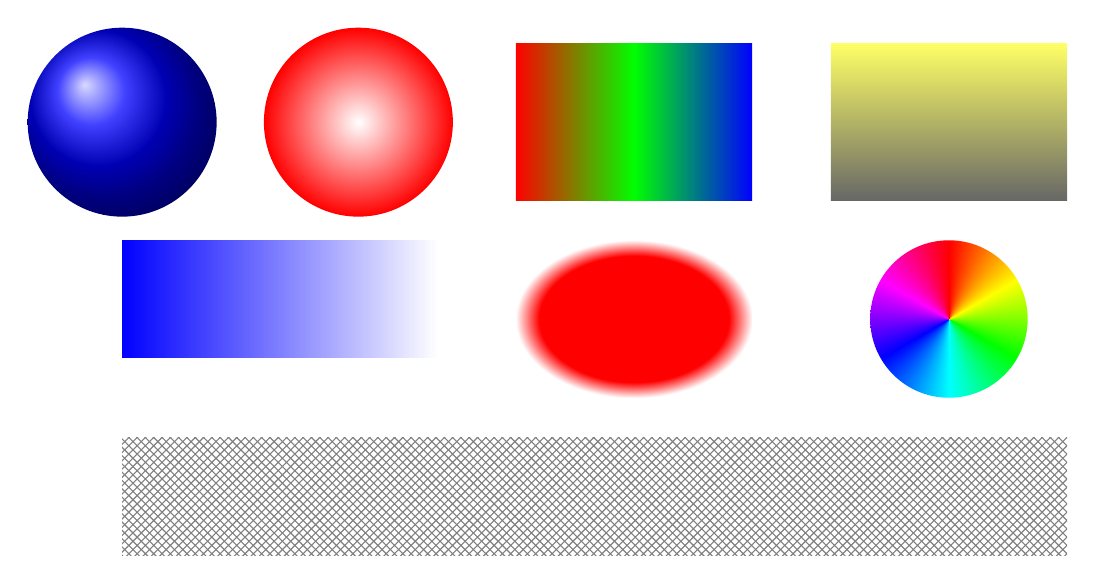
\begin{tikzpicture}
    \shade[ball color=blue] (0,0) circle (1.2);
    \shade[inner color=white,outer color=red] (3,0) circle (1.2);
    \shade[left color=red,right color=blue,middle color=green] (5,-1) rectangle (8,1);
    \shade[top color=yellow,bottom color=black,opacity=0.6] (9,-1) rectangle (12,1);
    \fill[blue,path fading=east] (0,-3) rectangle (4,-1.5);
    \fill[red,path fading=circle with fuzzy edge 20 percent] (5,-3.5) rectangle (8,-1.5);
    \shade[shading=color wheel] (10.5,-2.5) circle (1);
    \fill[pattern=crosshatch,pattern color=gray] (0,-5.5) rectangle (12,-4);
  \end{tikzpicture}
\end{frame}
\begin{frame}{Transparency: 2400 overlapping translucent discs}
  \centering
  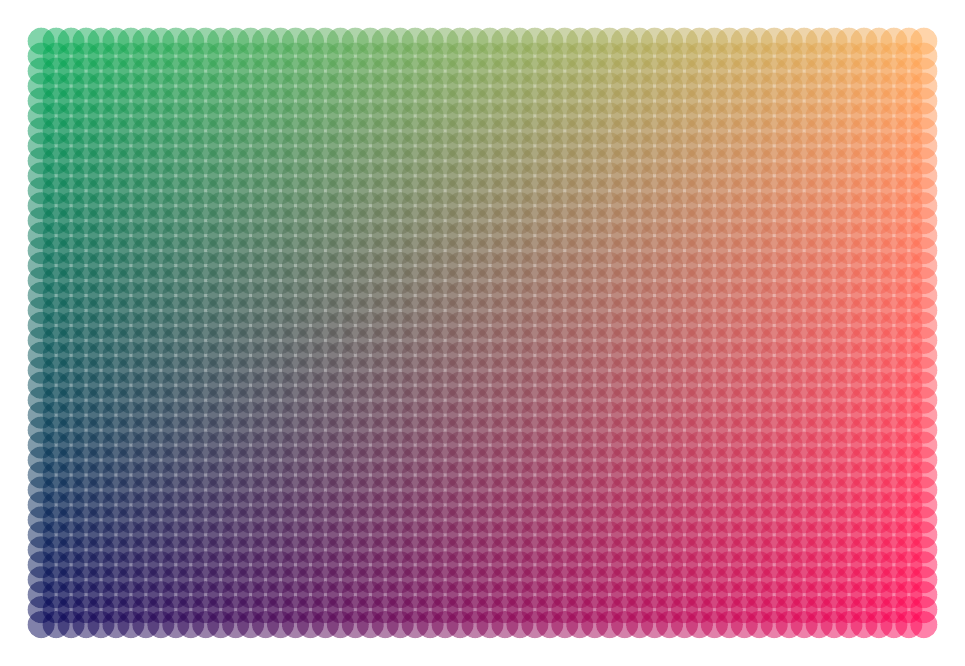
\begin{tikzpicture}[scale=0.19]
    \foreach \i in {1,...,60} {
      \foreach \j in {1,...,40} {
        \fill[opacity=0.5,color={rgb,60:red,\i;green,\j;blue,20}] (\i,\j) circle (0.9);
      }
    }
  \end{tikzpicture}
\end{frame}
\begin{frame}{Blend modes and transparency groups}
  \centering
  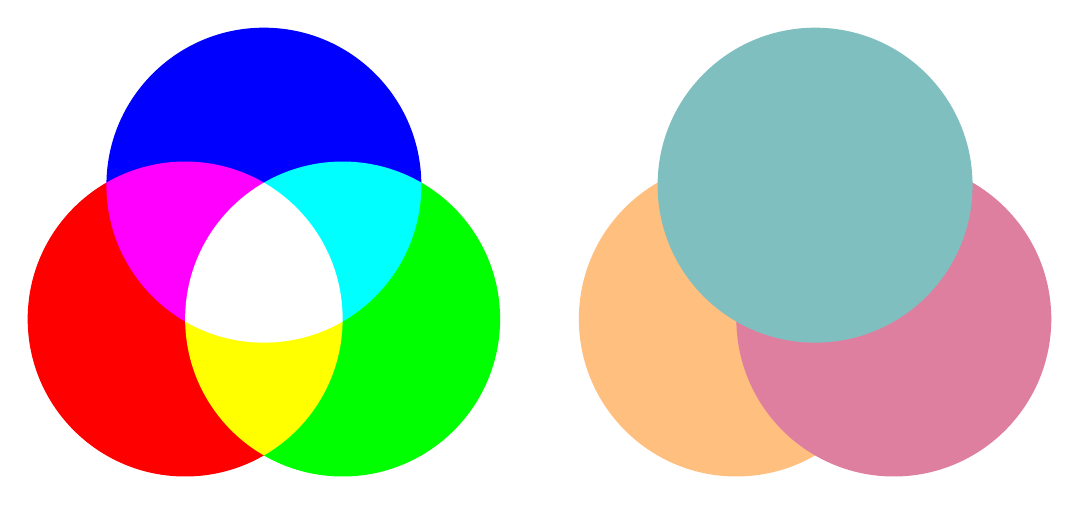
\begin{tikzpicture}
    \begin{scope}[blend group=screen]
      \fill[red] (0,0) circle (2);
      \fill[green] (2,0) circle (2);
      \fill[blue] (1,1.7) circle (2);
    \end{scope}
    \begin{scope}[xshift=7cm,transparency group,opacity=0.5]
      \fill[orange] (0,0) circle (2);
      \fill[purple] (2,0) circle (2);
      \fill[teal] (1,1.7) circle (2);
    \end{scope}
  \end{tikzpicture}
\end{frame}
\begin{frame}{Scatter with colour mapping and a dense mesh}
  \centering
  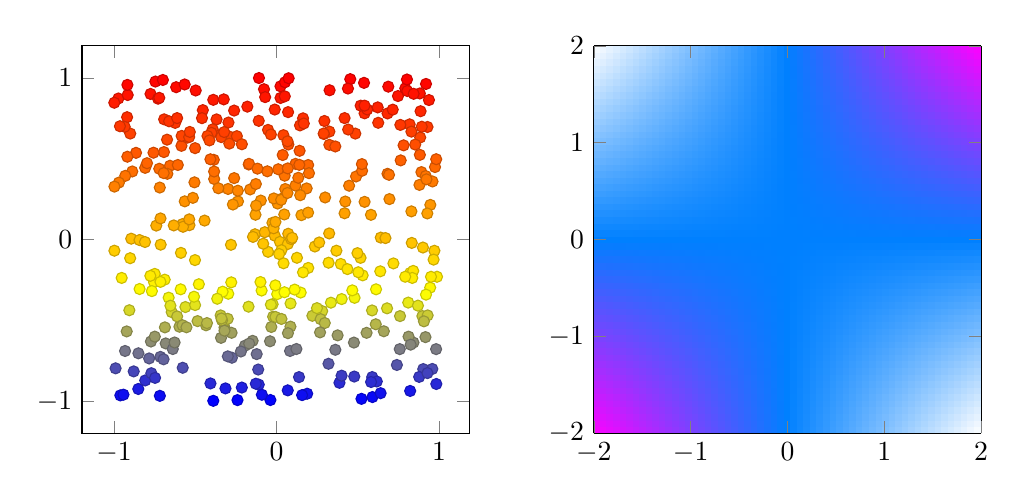
\begin{tikzpicture}
    \begin{axis}[width=6.5cm,height=6.5cm,colormap/hot]
      \addplot[scatter,only marks,mark=*,point meta=y,samples=400,domain=0:1] ({rand},{rand});
    \end{axis}
    \begin{axis}[width=6.5cm,height=6.5cm,xshift=6.5cm,view={0}{90},colormap/cool]
      \addplot3[surf,shader=flat,samples=60,domain=-2:2] {x*y};
    \end{axis}
  \end{tikzpicture}
\end{frame}
\end{document}
